
\subsubsection{28.10.14}

\begin{enumerate}
	\item The time of beginning and ending of the meeting:
	17:00 - 19:00
	\item Purposes of the meeting:
	\begin{enumerate}
	  \item To finish MCB.
	  
    \end{enumerate}
    
	\item Work that has been done:
	\begin{enumerate}
	  \item Servo which rotates the beam must be fixed as low as possible for maximum accuracy of capture.
      
      \item It was decided to fix servo in the following way: make hole diametr as the shaft of the servo. It need for location the servo so that it doesn't go beyond the robot's body (otherwise the robot did not meet in regulated dimentions) and able to rotate freely.
      
      \item The hole was made.
      
      \begin{figure}[H]
      	\begin{minipage}[h]{0.31\linewidth}
      		\center{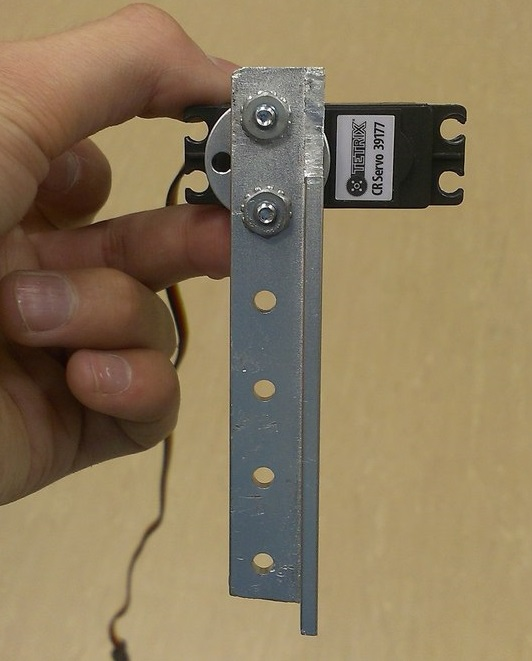
\includegraphics[scale=0.2]{days/28.10.14/images/01}}
      		\caption{Servo}
      	\end{minipage}
      	\hfill
      	\begin{minipage}[h]{0.31\linewidth}
      		\center{
\includegraphics[scale=0.15]{days/28.10.14/images/02}}
      		\caption{Hole for servo}
      	\end{minipage}
      	\hfill
      	\begin{minipage}[h]{0.31\linewidth}
      		\center{
\includegraphics[scale=0.15]{days/28.10.14/images/03}}
      		\caption{Planned mount}
      	\end{minipage}
      \end{figure}
      
    \end{enumerate}
    
	\item Results: 
	\begin{enumerate}
	  \item It was elaborated and partially implemented plan of fixing servo that rotates MCB.  
	  
    \end{enumerate}
    
	\item Tasks for the next meetings:
	\begin{enumerate}
	  \item To finish MCB.
	  
    \end{enumerate}     
\end{enumerate}
\fillpage
